\documentclass[10pt]{article}
\usepackage[polish]{babel}
\usepackage[utf8]{inputenc}
\usepackage[T1]{fontenc}
\usepackage{graphicx}
\usepackage[export]{adjustbox}
\graphicspath{ {./images/} }
\usepackage{amsmath}
\usepackage{amsfonts}
\usepackage{amssymb}
\usepackage[version=4]{mhchem}
\usepackage{stmaryrd}
\usepackage{multirow}

\title{EGZAMIN MATURALNY \\
 Z MATEMATYKI }

\author{}
\date{}


\newcommand\Varangle{\mathop{{<\!\!\!\!\!\text{\small)}}\:}\nolimits}

\begin{document}
\maketitle
Arkusz zawiera informacje prawnie chronione do momentu rozpoczęcia egzaminu.

UZUPELNIA ZDAJĄCY\\
KOD\\
PESEL\\
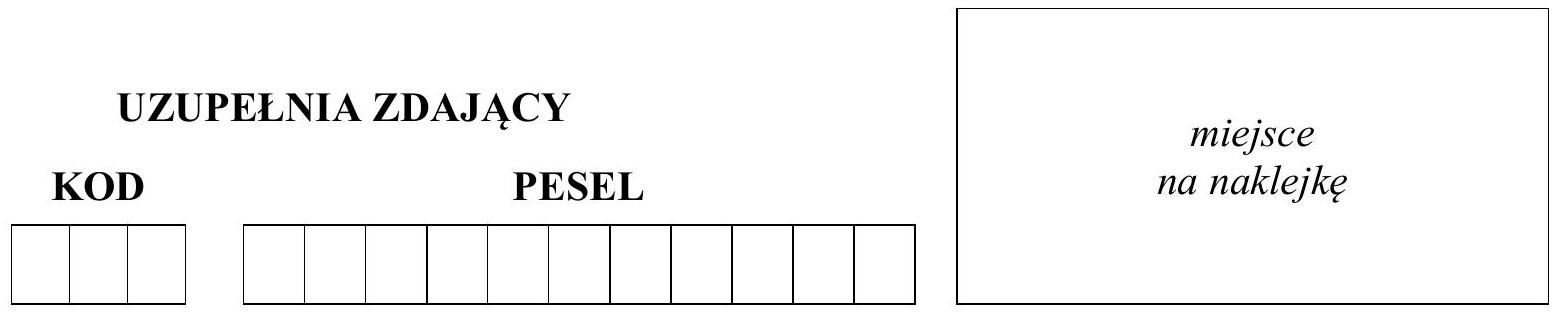
\includegraphics[max width=\textwidth, center]{2024_11_21_7379bf55d75dd0fc4c58g-01}

\section*{POZIOM ROZSZERZONY}
\section*{Instrukcja dla zdającego}
\begin{enumerate}
  \item Sprawdź, czy arkusz egzaminacyjny zawiera 20 stron (zadania 1-11). Ewentualny brak zgłoś przewodniczącemu zespołu nadzorującego egzamin.
  \item Rozwiązania zadań i odpowiedzi wpisuj w miejscu na to przeznaczonym.
  \item Pamiętaj, że pominięcie argumentacji lub istotnych obliczeń w rozwiązaniu zadania otwartego może spowodować, że za to rozwiązanie nie otrzymasz pełnej liczby punktów.
  \item Pisz czytelnie i używaj tylko długopisu lub pióra z czarnym tuszem lub atramentem.
  \item Nie używaj korektora, a błędne zapisy wyraźnie przekreśl.
  \item Pamiętaj, że zapisy w brudnopisie nie będą oceniane.
  \item Możesz korzystać z zestawu wzorów matematycznych, cyrkla i linijki oraz kalkulatora prostego.
  \item Na tej stronie oraz na karcie odpowiedzi wpisz swój numer PESEL i przyklej naklejkę z kodem.
  \item Nie wpisuj żadnych znaków w części przeznaczonej dla egzaminatora.
\end{enumerate}

\section*{UZUPELNIA ZESPÓŁ}
NADZORUJĄCY\\
Uprawnienia zdającego do:\\
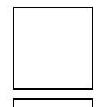
\includegraphics[max width=\textwidth, center]{2024_11_21_7379bf55d75dd0fc4c58g-01(1)}\\
dostosowania kryteriów oceniania\\
nieprzenoszenia zaznaczeń na kartę

9 MAJA 2018

Godzina rozpoczęcia:\\
9:00

Czas pracy:\\
180 minut

Liczba punktów do uzyskania: 50

MMA-R1\_1P-182

\section*{Zadanie 1. (4 pkt)}
Rozwiąż równanie \(3|x+2|=|x-3|+11\).\\

\includegraphics[max width=\textwidth, center]{2024_11_21_7379bf55d75dd0fc4c58g-02}\\

\includegraphics[max width=\textwidth, center]{2024_11_21_7379bf55d75dd0fc4c58g-03}

Odpowiedź:

\begin{center}
\begin{tabular}{|c|l|c|}
\hline
\multirow{2}{*}{\begin{tabular}{l}
Wypelnia \\
egzaminator \\
\end{tabular}} & Nr zadania & 1. \\
\cline { 2 - 3 }
 & Maks. liczba pkt & 4 \\
\cline { 2 - 3 }
 & Uzyskana liczba pkt &  \\
\hline
\end{tabular}
\end{center}

\section*{Zadanie 2. (5 pkt)}
Liczby \(a, b, c\), spełniające warunek \(3 a+b+3 c=77\), są odpowiednio pierwszym, drugim i trzecim wyrazem ciągu arytmetycznego. Ciąg \((a, b+1,2 c)\) jest geometryczny. Wyznacz liczby \(a, b, c\) oraz podaj wyrazy ciągu geometrycznego.\\

\includegraphics[max width=\textwidth, center]{2024_11_21_7379bf55d75dd0fc4c58g-04}\\

\includegraphics[max width=\textwidth, center]{2024_11_21_7379bf55d75dd0fc4c58g-05}

Odpowiedź:

\begin{center}
\begin{tabular}{|c|l|c|}
\hline
\multirow{2}{*}{\begin{tabular}{l}
Wypelnia \\
egzaminator \\
\end{tabular}} & Nr zadania & 2. \\
\cline { 2 - 3 }
 & Maks. liczba pkt & 5 \\
\cline { 2 - 3 }
 & Uzyskana liczba pkt &  \\
\hline
\end{tabular}
\end{center}

\section*{Zadanie 3. (5 pkt)}
Dany jest czworokąt wypukły \(A B C D\), w którym \(|A D|=|A B|=|B C|=a, \quad|\Varangle B A D|=60^{\circ}\) i \(|\Varangle A D C|=135^{\circ}\). Oblicz pole czworokąta \(A B C D\).\\

\includegraphics[max width=\textwidth, center]{2024_11_21_7379bf55d75dd0fc4c58g-06}\\

\includegraphics[max width=\textwidth, center]{2024_11_21_7379bf55d75dd0fc4c58g-07}

Odpowiedź:

\begin{center}
\begin{tabular}{|c|l|c|}
\hline
\multirow{2}{*}{\begin{tabular}{l}
Wypełnia \\
egzaminator \\
\end{tabular}} & Nr zadania & 3. \\
\cline { 2 - 3 }
 & Maks. liczba pkt & 5 \\
\cline { 2 - 3 }
 & Uzyskana liczba pkt &  \\
\hline
\end{tabular}
\end{center}

\section*{Zadanie 4. (4 pkt)}
Z liczb ośmioelementowego zbioru \(Z=\{1,2,3,4,5,6,7,9\}\) tworzymy ośmiowyrazowy ciąg, którego wyrazy nie powtarzają się. Oblicz prawdopodobieństwo zdarzenia polegającego na tym, że żadne dwie liczby parzyste nie są sąsiednimi wyrazami utworzonego ciągu. Wynik przedstaw w postaci ułamka zwykłego nieskracalnego.\\

\includegraphics[max width=\textwidth, center]{2024_11_21_7379bf55d75dd0fc4c58g-08}\\

\includegraphics[max width=\textwidth, center]{2024_11_21_7379bf55d75dd0fc4c58g-09}

Odpowiedź:

\begin{center}
\begin{tabular}{|c|l|c|}
\hline
\multirow{2}{*}{\begin{tabular}{c}
Wypełnia \\
egzaminator \\
\end{tabular}} & Nr zadania & 4. \\
\cline { 2 - 3 }
 & Maks. liczba pkt & 4 \\
\cline { 2 - 3 }
 & Uzyskana liczba pkt &  \\
\hline
\end{tabular}
\end{center}

\section*{Zadanie 5. (3 pkt)}
Trójkąt \(A B C\) jest ostrokątny oraz \(|A C|>|B C|\). Dwusieczna \(d_{C}\) kąta \(A C B\) przecina bok \(A B\) w punkcie \(K\). Punkt \(L\) jest obrazem punktu \(K\) w symetrii osiowej względem dwusiecznej \(d_{A}\) kąta \(B A C\), punkt \(M\) jest obrazem punktu \(L\) w symetrii osiowej względem dwusiecznej \(d_{C}\) kąta \(A C B\), a punkt \(N\) jest obrazem punktu \(M\) w symetrii osiowej względem dwusiecznej \(d_{B}\) kąta \(A B C\) (zobacz rysunek).\\
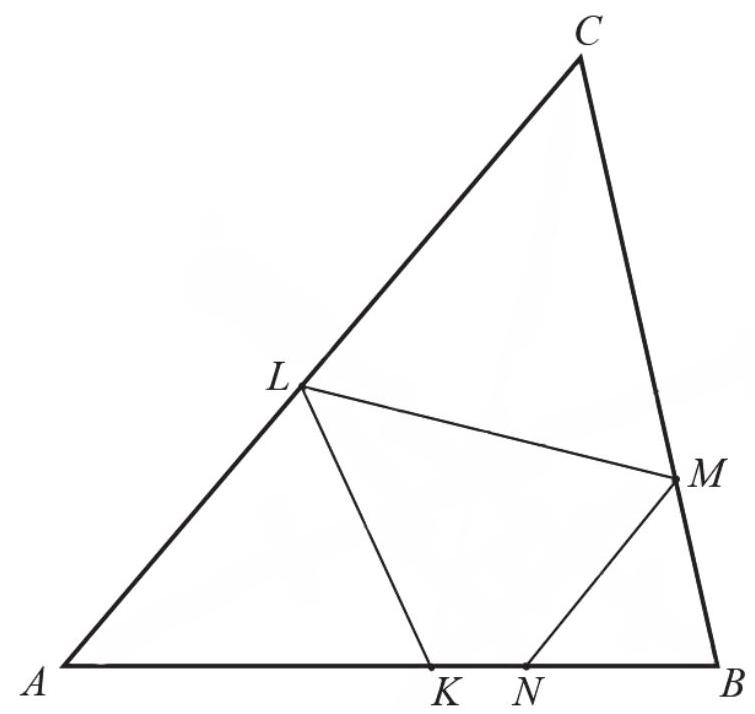
\includegraphics[max width=\textwidth, center]{2024_11_21_7379bf55d75dd0fc4c58g-10}

Udowodnij, że na czworokącie \(K N M L\) można opisać okrąg.\\

\includegraphics[max width=\textwidth, center]{2024_11_21_7379bf55d75dd0fc4c58g-10(1)}

\section*{Zadanie 6. (3 pkt)}
Udowodnij, że dla każdej liczby całkowitej \(k\) i dla każdej liczby całkowitej \(m\) liczba \(k^{3} m-\mathrm{km}^{3}\) jest podzielna przez 6.\\

\includegraphics[max width=\textwidth, center]{2024_11_21_7379bf55d75dd0fc4c58g-11}

\begin{center}
\begin{tabular}{|c|l|c|c|}
\hline
\multirow{2}{*}{\begin{tabular}{c}
Wypelnia \\
egzaminator \\
\end{tabular}} & Nr zadania & \(\mathbf{5 .}\) & \(\mathbf{6 .}\) \\
\cline { 2 - 4 }
 & Maks. liczba pkt & \(\mathbf{3}\) & \(\mathbf{3}\) \\
\cline { 2 - 4 }
 & Uzyskana liczba pkt &  &  \\
\hline
\end{tabular}
\end{center}

\section*{Zadanie 7. (4 pkt)}
Rozwiąż równanie \(2 \cos ^{2} x+3 \sin x=0\) w przedziale \(\left\langle-\frac{\pi}{2}, \frac{3 \pi}{2}\right\rangle\).\\

\includegraphics[max width=\textwidth, center]{2024_11_21_7379bf55d75dd0fc4c58g-12}

Odpowiedź: \(\qquad\)

\section*{Zadanie 8. (5 pkt)}
Liczba \(\frac{2}{5}\) jest pierwiastkiem wielomianu \(W(x)=5 x^{3}-7 x^{2}-3 x+p\). Wyznacz pozostałe pierwiastki tego wielomianu i rozwiąż nierówność \(W(x)>0\).\\

\includegraphics[max width=\textwidth, center]{2024_11_21_7379bf55d75dd0fc4c58g-13}

Odpowiedź:

\begin{center}
\begin{tabular}{|c|l|c|c|}
\hline
\multirow{2}{*}{\begin{tabular}{c}
Wypetnia \\
egzaminator \\
\end{tabular}} & Nr zadania & 7. & 8. \\
\cline { 2 - 4 }
 & Maks. liczba pkt & 4 & 5 \\
\cline { 2 - 4 }
 & Uzyskana liczba pkt &  &  \\
\hline
\end{tabular}
\end{center}

Zadanie 9. (6 pkt)\\
Wyznacz wszystkie wartości parametru \(m\), dla których równanie \(x^{2}+(m+1) x-m^{2}+1=0\) ma dwa rozwiązania rzeczywiste \(x_{1}\) i \(x_{2}\left(x_{1} \neq x_{2}\right)\), spełniające warunek \(x_{1}^{3}+x_{2}^{3}>-7 x_{1} x_{2}\).

\begin{center}
\begin{tabular}{|c|c|c|c|c|c|c|c|c|c|c|c|c|c|c|c|c|c|c|c|c|c|c|}
\hline
 &  &  &  &  &  &  &  &  &  &  &  &  &  &  &  &  &  &  &  &  &  &  \\
\hline
 &  &  &  &  &  &  &  &  &  &  &  &  &  &  &  &  &  &  &  &  &  &  \\
\hline
 &  &  &  &  &  &  &  &  &  &  &  &  &  &  &  &  &  &  &  &  &  &  \\
\hline
 &  &  &  &  &  &  &  &  &  &  &  &  &  &  &  &  &  &  &  &  &  &  \\
\hline
 &  &  &  &  &  &  &  &  &  &  &  &  &  &  &  &  &  &  &  &  &  &  \\
\hline
 &  &  &  &  &  &  &  &  &  &  &  &  &  &  &  &  &  &  &  &  &  &  \\
\hline
 &  &  &  &  &  &  &  &  &  &  &  &  &  &  &  &  &  &  &  &  &  &  \\
\hline
 &  &  &  &  &  &  &  &  &  &  &  &  &  &  &  &  &  &  &  &  &  &  \\
\hline
 &  &  &  &  &  &  &  &  &  &  &  &  &  &  &  &  &  &  &  &  &  &  \\
\hline
 &  &  &  &  &  &  &  &  &  &  &  &  &  &  &  &  &  &  &  &  &  &  \\
\hline
 &  &  &  &  &  &  &  &  &  &  &  &  &  &  &  &  &  &  &  &  &  &  \\
\hline
 &  &  &  &  &  &  &  &  &  &  &  &  &  &  &  &  &  &  &  &  &  &  \\
\hline
 &  &  &  &  &  &  &  &  &  &  &  &  &  &  &  &  &  &  &  &  &  &  \\
\hline
 &  &  &  &  &  &  &  &  &  &  &  &  &  &  &  &  &  &  &  &  &  &  \\
\hline
 &  &  &  &  &  &  &  &  &  &  &  &  &  &  &  &  &  &  &  &  &  &  \\
\hline
 &  &  &  &  &  &  &  &  &  &  &  &  &  &  &  &  &  &  &  &  &  &  \\
\hline
 &  &  &  &  &  &  &  &  &  &  &  &  &  &  &  &  &  &  &  &  &  &  \\
\hline
 &  &  &  &  &  &  &  &  &  &  &  &  &  &  &  &  &  &  &  &  &  &  \\
\hline
 &  &  &  &  &  &  &  &  &  &  &  &  &  &  &  &  &  &  &  &  &  &  \\
\hline
 &  &  &  &  &  &  &  &  &  &  &  &  &  &  &  &  &  &  &  &  &  &  \\
\hline
 &  &  &  &  &  &  &  &  &  &  &  &  &  &  &  &  &  &  &  &  &  &  \\
\hline
 &  &  &  &  &  &  &  &  &  &  &  &  &  &  &  &  &  &  &  &  &  &  \\
\hline
 &  &  &  &  &  &  &  &  &  &  &  &  &  &  &  &  &  &  &  &  &  &  \\
\hline
 &  &  &  &  &  &  &  &  &  &  &  &  &  &  &  &  &  &  &  &  &  &  \\
\hline
 &  &  &  &  &  &  &  &  &  &  &  &  &  &  &  &  &  &  &  &  &  &  \\
\hline
 &  &  &  &  &  &  &  &  &  &  &  &  &  &  &  &  &  &  &  &  &  &  \\
\hline
 &  &  &  &  &  &  &  &  &  &  &  &  &  &  &  &  &  &  &  &  &  &  \\
\hline
 &  &  &  &  &  &  &  &  &  &  &  &  &  &  &  &  &  &  &  &  &  &  \\
\hline
 &  &  &  &  &  &  &  &  &  &  &  &  &  &  &  &  &  &  &  &  &  &  \\
\hline
 &  &  &  &  &  &  &  &  &  &  &  &  &  &  &  &  &  &  &  &  &  &  \\
\hline
 &  &  &  &  &  &  &  &  &  &  &  &  &  &  &  &  &  &  &  &  &  &  \\
\hline
 &  &  &  &  &  &  &  &  &  &  &  &  &  &  &  &  &  &  &  &  &  &  \\
\hline
 &  &  &  &  &  &  &  &  &  &  &  &  &  &  &  &  &  &  &  &  &  &  \\
\hline
 &  &  &  &  &  &  &  &  &  &  &  &  &  &  &  &  &  &  &  &  &  &  \\
\hline
 &  &  &  &  &  &  &  &  &  &  &  &  &  &  &  &  &  &  &  &  &  &  \\
\hline
 &  &  &  &  &  &  &  &  &  &  &  &  &  &  &  &  &  &  &  &  &  &  \\
\hline
 &  &  &  &  &  &  &  &  &  &  &  &  &  &  &  &  &  &  &  &  &  &  \\
\hline
 &  &  &  &  &  &  &  &  &  &  &  &  &  &  &  &  &  &  &  &  &  &  \\
\hline
 &  &  &  &  &  &  &  &  &  &  &  &  &  &  &  &  &  &  &  &  &  &  \\
\hline
 &  &  &  &  &  &  &  &  &  &  &  &  &  &  &  &  &  &  &  &  &  &  \\
\hline
 &  &  &  &  &  &  &  &  &  &  &  &  &  &  &  &  &  &  &  &  &  &  \\
\hline
 &  &  &  &  &  &  &  &  &  &  &  &  &  &  &  &  &  &  &  &  &  &  \\
\hline
 &  &  &  &  &  &  &  &  &  &  &  &  &  &  &  &  &  &  &  &  &  &  \\
\hline
 &  &  &  &  &  &  &  &  &  &  &  &  &  &  &  &  &  &  &  &  &  &  \\
\hline
\end{tabular}
\end{center}

\begin{center}

\includegraphics[max width=\textwidth]{2024_11_21_7379bf55d75dd0fc4c58g-15}
\end{center}

Odpowiedź:

\begin{center}
\begin{tabular}{|c|l|c|}
\hline
\multirow{2}{*}{\begin{tabular}{c}
Wypełnia \\
egzaminator \\
\end{tabular}} & Nr zadania & 9. \\
\cline { 2 - 3 }
 & Maks. liczba pkt & \(\mathbf{6}\) \\
\cline { 2 - 3 }
 & Uzyskana liczba pkt &  \\
\hline
\end{tabular}
\end{center}

\section*{Zadanie 10. (6 pkt)}
Punkt \(A=(7,-1)\) jest wierzchołkiem trójkąta równoramiennego \(A B C\), w którym \(|A C|=|B C|\). Obie współrzędne wierzchołka \(C\) są liczbami ujemnymi. Okrąg wpisany w trójkąt \(A B C\) ma równanie \(x^{2}+y^{2}=10\). Oblicz współrzędne wierzchołków \(B\) i \(C\) tego trójkąta.\\

\includegraphics[max width=\textwidth, center]{2024_11_21_7379bf55d75dd0fc4c58g-16}\\

\includegraphics[max width=\textwidth, center]{2024_11_21_7379bf55d75dd0fc4c58g-17}

Odpowiedź:

\begin{center}
\begin{tabular}{|c|l|c|}
\hline
\multirow{2}{*}{\begin{tabular}{l}
Wypelnia \\
egzaminator \\
\end{tabular}} & Nr zadania & 10. \\
\cline { 2 - 3 }
 & Maks. liczba pkt & \(\mathbf{6}\) \\
\cline { 2 - 3 }
 & Uzyskana liczba pkt &  \\
\hline
\end{tabular}
\end{center}

\section*{Zadanie 11. (5 pkt)}
Przekrój ostrosłupa prawidłowego trójkątnego \(A B C S\) płaszczyzną przechodzącą przez wierzchołek \(S\) i wysokości dwóch ścian bocznych jest trójkątem równobocznym. Krawędź boczna tego ostrosłupa ma długość \(\frac{4 \sqrt{3}}{3}\). Oblicz objętość tego ostrosłupa.\\

\includegraphics[max width=\textwidth, center]{2024_11_21_7379bf55d75dd0fc4c58g-18}\\

\includegraphics[max width=\textwidth, center]{2024_11_21_7379bf55d75dd0fc4c58g-19}

Odpowiedź: \(\qquad\)

\begin{center}
\begin{tabular}{|c|l|c|}
\hline
\multirow{2}{*}{\begin{tabular}{l}
Wypelnia \\
egzaminator \\
\end{tabular}} & Nr zadania & 11. \\
\cline { 2 - 3 }
 & Maks. liczba pkt & 5 \\
\cline { 2 - 3 }
 & Uzyskana liczba pkt &  \\
\hline
\end{tabular}
\end{center}

\section*{BRUDNOPIS (nie podlega ocenie)}

\end{document}